\documentclass[
    11pt,
    spanish,
    a4paper
]{article}
%\usepackage[a4paper,left=.4in,right=.4in,top=1in,bottom=1in]{geometry}
\usepackage[utf8]{inputenc}
\usepackage[spanish]{babel}
\usepackage{authoraftertitle}
\usepackage{booktabs}
\usepackage{breqn}
\usepackage{caption}
\usepackage{float}
\usepackage{graphicx}
\usepackage{listings}
\usepackage{verbatim}

\def\doctype{Trabajo práctico}
\title{Ejercicios de FT \& RDB}
\author{Gonzalo Nahuel Vaca}

\begin{document}

\makeatletter
\begin{titlepage}
	\begin{center}
		\vspace*{1cm}

		\Huge
		\textbf{\doctype}
		\vspace{0.5cm}

		\LARGE
		\@title
		\vspace{0.5cm}

		\textbf{Introducción a los sistemas críticos}

		\vspace{1.5cm}

		\textbf{\@author}

		\vspace{1.5cm}

		
\includegraphics[width=0.8\textwidth]{img/logoFIUBA.pdf}

		\vfill
		Maestría en Sistemas Embebidos\\
		Universidad de Buenos Aires\\
		Argentina\\
		\today
	\end{center}
\end{titlepage}
\makeatother
\newpage

\section{Ejercicio 1}

En la figura \ref{fig:rdboriginal} se observa el RDB del ejercicio.

\begin{figure}[htbp]
	\centering
	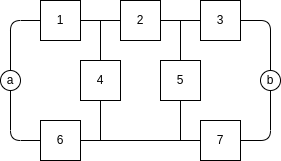
\includegraphics[width=0.4\textwidth]{img/rdb.png}
	\caption{RDB del ejercicio.}
	\label{fig:rdboriginal}
\end{figure}

A partir de la figura \ref{fig:rdboriginal} se identificaron los caminos posibles:

$$ C_1 = R_1 . R_2 . R_3 $$
$$ C_2 = R_1 . R_4 . R_7 $$
$$ C_3 = R_1 . R_4 . R_5 . R_3 $$
$$ C_4 = R_6 . R_7 $$
$$ C_5 = R_6 . R_5 . R_3 $$
$$ C_6 = R_6 . R_4 . R_2 .R_3 $$
$$ C_7 = R_1 . R_2 . R_5 .R_7 $$

Finalmente el RDB paralelo queda de la siguiente manera:

\begin{figure}[htbp]
	\centering
	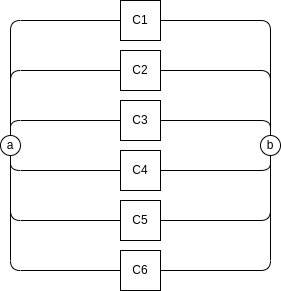
\includegraphics[width=0.4\textwidth]{img/rdb_paralelo.png}
	\caption{RDB paralelo.}
	\label{fig:rdbparalelo}
\end{figure}

\begin{dmath}
	\theta = 1 - ((1 - C_1).(1-C_2).(1-C_3).(1-C_4).(1-C_5).(1-C_6).(1-C_7))
\end{dmath}

\section{Ejercicio 2}

En la figura \ref{fig:rdbequivalente} se puede observar un modelo RDB equivalente.

\begin{figure}[htbp]
	\centering
	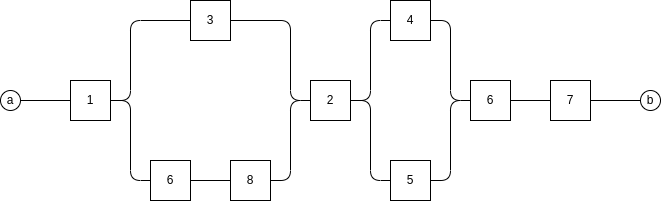
\includegraphics[width=\textwidth]{img/rdb2.png}
	\caption{RDB del equivalente.}
	\label{fig:rdbequivalente}
\end{figure}

A continuación se observa su función de estructura:

\begin{dmath}
	\theta = (X_2 . (1 - (1-X_3).(1-(X_6.X_8)))) . ((X_6 . X_7) . (1-(1-X_4).(1-X_5))) . X_1
\end{dmath}

\newpage

\section{Ejercicio 3}

En la figura \ref{fig:fotoradar} se puede observar una fotografía de un Radar de Vigilancia Primario.

\begin{figure}[htbp]
	\centering
	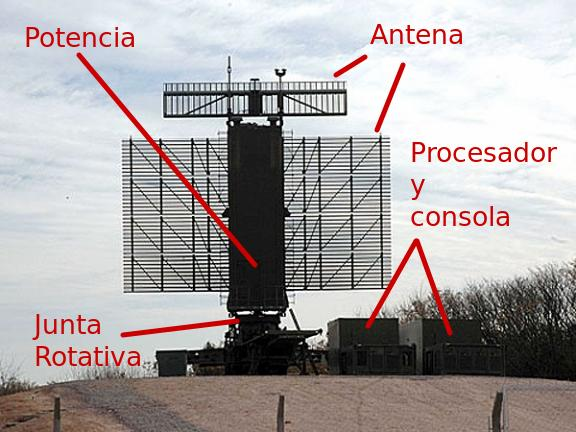
\includegraphics[width=0.8\textwidth]{img/radares.jpg}
	\caption{Fotografía del radar.}
	\label{fig:fotoradar}
\end{figure}

En la figura \ref{fig:radar} se puede observar el diagrama esquemático de un Radar de Vigilancia Primario.

\begin{figure}[htbp]
	\centering
	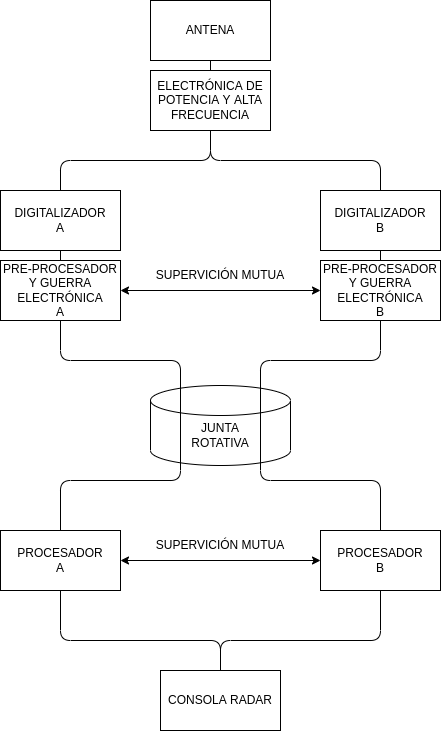
\includegraphics[width=0.5\textwidth]{img/radar.png}
	\caption{Diagrama del radar.}
	\label{fig:radar}
\end{figure}

Por encima de la junta rotativa se encuentran los componentes que giran en azimut mientras que debajo se encuentran los componentes estáticos.

\begin{figure}[htbp]
	\centering
	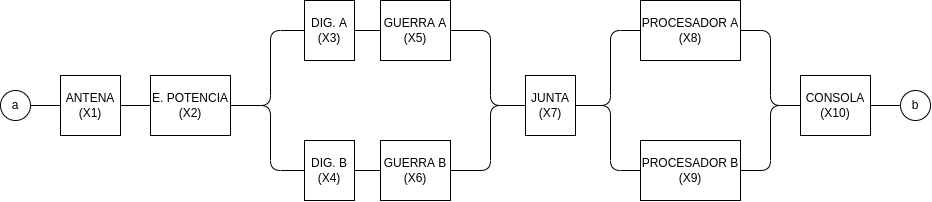
\includegraphics[width=\textwidth]{img/rdb_radar.png}
	\caption{RDB del radar.}
	\label{fig:rdb_radar}
\end{figure}


\begin{dmath}
	\theta = x_1 . x_2 . (1 - ((1 - (x_3 . x_5)) . (1-(x_4 . x_6)) )) . x_7 . (1 - ((1 - x_8).(1 - x_9))) . x_{10}
\end{dmath}

En la figura \ref{fig:arbol} se puede observar el árbol de fallas.

\begin{figure}[htbp]
	\centering
	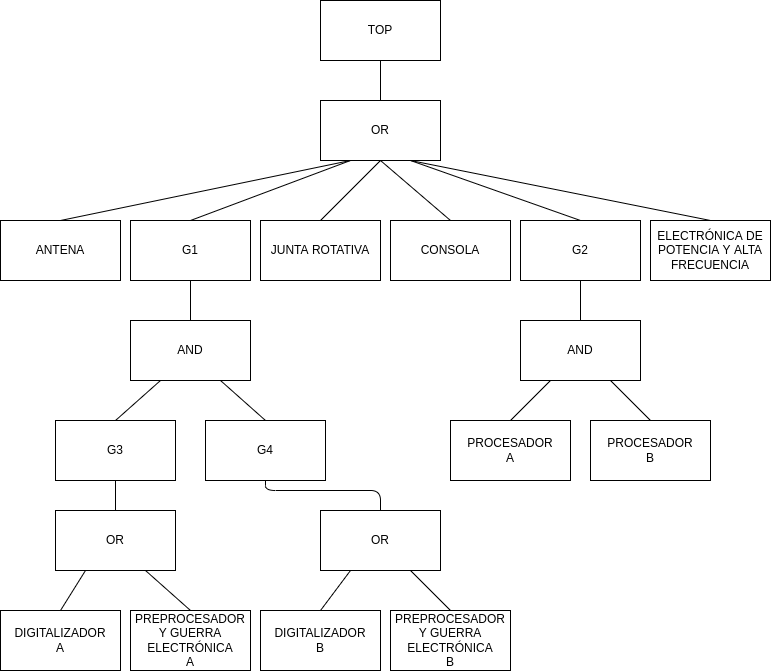
\includegraphics[width=0.8\textwidth]{img/arbol_radar.png}
	\caption{Árbol de falla.}
	\label{fig:arbol}
\end{figure}

\end{document}